% !TeX TXS-program:compile = txs:///pdflatex/[--shell-escape]
\documentclass[handout, aspectratio=169, 10pt]{beamer}

% packages
\usepackage{newpxmath} % math font is Palatino compatible
% \usepackage[nomath]{fontspec}

\usepackage{setspace}
\usepackage{xcolor}
\usepackage{soul} % for \st
\usepackage{hyperref} % for links
\definecolor{links}{HTML}{2A1B81}
\hypersetup{colorlinks,linkcolor=,urlcolor=links}


% table stuff
\usepackage{chronosys}
\usepackage{verbatim}
% \pagenumbering{arabic}
\usepackage{tabularx}
\usepackage{booktabs}
\usepackage{ragged2e}
\usepackage{mathtools}

% R Code
\usepackage{listings}
\usepackage{courier}
\lstset{basicstyle=\scriptsize\ttfamily,breaklines=true}
\lstset{framextopmargin=50pt,frame=bottomline}

% themes
\usetheme[progressbar=frametitle, block=fill]{metropolis}
\useoutertheme{metropolis}
\useinnertheme{metropolis}

% colors
\definecolor{dimwhite}{rgb}{0.99, 0.99, 0.99}
\definecolor{charcoal}{rgb}{0.21, 0.27, 0.31}
\definecolor{slategray}{rgb}{0.44, 0.5, 0.56}
\definecolor{dimgray}{rgb}{0.41, 0.41, 0.41}
\definecolor{bleudefrance}{rgb}{0.19, 0.55, 0.91}

% beamer options
\setbeamercolor{author}{fg=charcoal}
\setbeamercolor{background canvas}{bg=white}
\setbeamercolor{section in toc}{fg=charcoal}
\setbeamercolor{subsection in toc}{fg=dimgray}
\setbeamercolor{frametitle}{bg=dimwhite, fg=charcoal}
\setbeamercolor{progress bar}{fg=slategray, bg=fg!50!black!30}
\setbeamercovered{transparent}
\setbeamertemplate{itemize items}[triangle]
\setbeamertemplate{itemize subitem}[circle]
\setbeamertemplate{itemize subsubitem}[square]
\setbeamersize{text margin left=7mm,text margin right=7mm} 

% new commands
\newcommand{\q}[1]{``#1''}
\newcommand{\hs}[1]{\textsc{\hfill\scriptsize\color{dimgray}#1}}
\newcommand{\g}[1]{{\color{gray}#1}}
\newcommand{\dg}[1]{{\color{dimgray}#1}}
\newcommand{\sg}[1]{{\color{slategray}#1}}
\newcommand{\bdf}[1]{{\color{bleudefrance}#1}}
\newcommand{\itemcolor}[1]{\renewcommand{\makelabel}[1]{\color{#1}\hfil ##1}}
\newcommand\Wider[2][2em]{
\makebox[\linewidth][c]{
  \begin{minipage}{\dimexpr\textwidth+#1\relax}
  \raggedright#2
  \end{minipage}
  }
}

% misc
\linespread{1.35}

% minted (risky)
\usepackage[cache=false]{minted}

% Math stuff
\newcommand{\norm}[1]{\left\lVert#1\right\rVert}
\newcommand{\R}{\mathbb{R}}
\newcommand{\E}{\mathbb{E}}
\newcommand{\V}{\mathbb{V}}
\newcommand{\probP}{\text{I\kern-0.15em P}}
\newcommand{\ol}{\overline}
%\newcommand{\ul}{\underline}
\newcommand{\pp}{{\prime \prime}}
\newcommand{\ppp}{{\prime \prime \prime}}
\newcommand{\policy}{\gamma}
\newcommand{\plim}{ \overset{p}{\to}}
\newcommand{\hnot}{ \overset{H_0}{\to}}

% Causal Graphs
\usetikzlibrary{shapes,decorations,arrows,calc,arrows.meta,fit,positioning}
\tikzset{
    -Latex,auto,node distance =1 cm and 1 cm,semithick,
    state/.style ={ellipse, draw, minimum width = 0.7 cm},
    point/.style = {circle, draw, inner sep=0.04cm,fill,node contents={}},
    bidirected/.style={Latex-Latex,dashed},
    el/.style = {inner sep=2pt, align=left, sloped}
}

\setbeamersize{text margin left=10pt,text margin right=10pt}


\begin{document}


\title[L4 - Inference and Standard Errors]{ Econometrics I}
\subtitle{Lecture 4: Inference and Standard Errors}
\author{Chris Conlon}
\date{Fall 2025}
\maketitle


\begin{frame}
\begin{center}
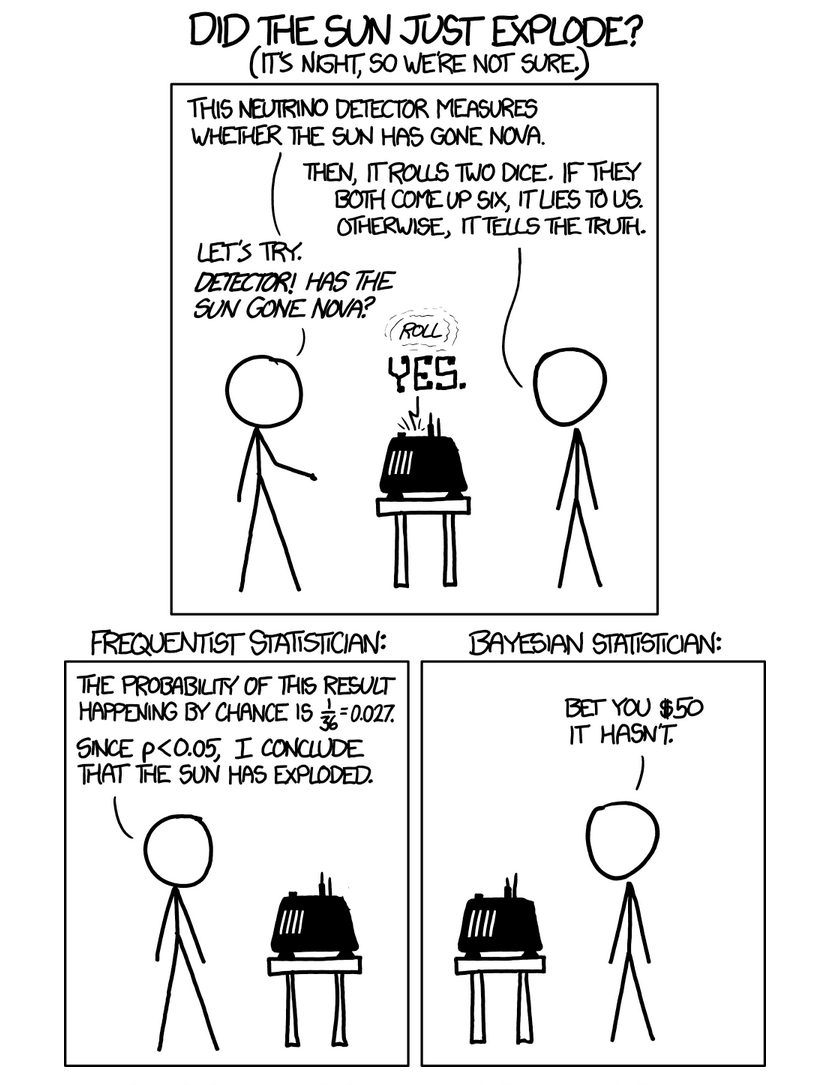
\includegraphics[height=.92\textheight]{explode} \\
{\tiny Source: xkcd.com}
\end{center}
\end{frame}



\section{Recap: Asymptotics for OLS and the Linear Model}


\begin{frame}{OLS}
\begin{align*}
y_i = \beta_0 + \beta x_i + u_i
\end{align*}
Recall the three basic OLS assumptions
\begin{enumerate}
\item $\mathbb{E}(u_i |X_i ) = 0$
\item $(X_i,Y_i)$, $i =1,\ldots,n$, are i.i.d.
\item Large outliers are rare $\mathbb{E}[Y^4]< \infty$ and $\mathbb{E}[X^4]<\infty$.
\end{enumerate}
\end{frame}

\begin{frame}{Unbiasedness and Consistency}
\begin{itemize}
\item Unbiasedness means on average we don't over or under estimate $\widehat{\beta}$
\begin{align*}
\E[\widehat{\beta} ] - \beta_0 = 0
\end{align*}
\item Consistency tells us that we approach the true $\beta_0$ as $n \rightarrow \infty$.
\begin{align*}
\widehat{\beta}  \overset{p}{\to} \beta_0
\end{align*}
\item Example: $X_{(1)}$ is unbiased but not consistent for the mean.
\item Example $\frac{n}{n-5} \overline{X}$ is consistent but biased for the mean.
\end{itemize}
\end{frame}



\begin{frame}{Outliers}
\begin{itemize}
	\item {\bf Outliers} refer to observations that are ``far away'' from the rest of the data. 
	They can be due to errors in the data.  There is no standard formal definition. 

	\medskip
	\item What to do? Greene:``\emph{It is difficult to draw firm general conclusions... It remains likely that in very
	small samples, some caution and close scrutiny of the data are called for.}'' I'd say that's true even in large samples,
	but there isn't a generally accepted way of quantifying what counts as appropriate ``caution and close scrutiny.''


\end{itemize}
\end{frame}


\begin{frame}{Removing Outliers?}
\begin{itemize}
\item Removing extreme outliers (in $x$) from datasets is often considered good practice. But we should be mindful
		about why as dropping observations creates the potential for manipulation. 

	\medskip
	\item Sometimes extreme outliers are just errors, in which case they should almost certainly be dropped.

	\medskip
	\item Even if they aren't errors, they may reflect a different mode in the data generating process. They may require
		a different or more general model to account for them properly. Consider the justificaiton of a linear
		model based on Taylor's theorem (local linear approximation). With such a justification for your modeling
		strategy, it would not make sense to include an outlier in $x$.
	\medskip
	\item It's important to be transparent about how dropped outliers affect results. 

\end{itemize}
\end{frame}




\begin{frame}{Outliers and Leverage}
\begin{itemize}
\item One way to find influential observations is to calculate the {\bf leverage} of each observation $i$. We begin with the hat matrix:
\begin{align*}
P = {\bf X} ({\bf X} '{\bf X})^{-1}  {\bf X}'
\end{align*}
and consider the diagonal elements, which are labeled $h_{ii}$
\begin{align*}
h_{ii} = \bf{x}_i `({\bf X} '{\bf X})^{-1}  \bf{x}_i
\end{align*}

\medskip
\item This tells us how influential an observation is in our estimate of ${\bf b}_{OLS}$.\\
Particularly important for $\{0,1\}$ dummy variables with uneven groups.
\end{itemize}
\end{frame}



\begin{frame}{Leave One Out Regression}
\begin{itemize}
\item This is sometimes called the {\bf Jackknife}
\item Sometimes it is helpful to know what would happen if we omitted a single observation $i$
\item Turns out we don't need to run $N$ regressions
\begin{align*}
{\bf b}_{-i} &= ({\bf X}_{-i}'{\bf X}_{-i})^{-1} {\bf X}_{-i}' {\bf y}_{-i} \\
&={\bf b}_{OLS} -  ({\bf X} '{\bf X})^{-1} {\bf x}_i  \tilde{e}_i  \quad \mbox{ where } \tilde{e}_i = (1-h_{ii})^{-1} e_i
\end{align*}
\item $\tilde{e}_i $ has the interpretation of the LOO prediction error.
\item high leverage observations move ${\bf b}_{OLS}$ a lot.
\end{itemize}
\end{frame}


% \begin{frame}{Outliers and Leverage}
% One way to find \alert{outliers} is to calculate the \alert{leverage} of each observation $i$. We begin with the \alert{hat matrix}:
% \begin{align*}
% P = X  (X'X)^{-1} X'
% \end{align*}
% and consider the diagonal elements which for some reason are labeled $h_{ii}$
% \begin{align*}
% h_{ii} = x_i (X'X)^{-1} x_i'
% \end{align*}
% This tells us how \alert{influential} an observation is in our estimate of $\widehat{\beta}$.\\
% Particularly important for $\{0,1\}$ \alert{dummy variables} with uneven groups.
% \end{frame}


% \begin{frame}{Leave One Out Regression}
% \begin{itemize}
% \item This is sometimes called the \alert{Jackknife}
% \item Sometimes it is helpful to know what would happen if we omitted a single observation $i$
% \item Turns out we don't need to run $N$ regressions
% \begin{align*}
% \widehat{\beta}_{-i} &= (X_{-i}'X_{-i})^{-1} X_{-i}' Y_{-i} \\
% &=\widehat{\beta} -  (X 'X)^{-1} x_i  \tilde{u}_i  \quad \mbox{ where } \tilde{u}_i = (1-h_{ii})^{-1}\hat{u}_i
% \end{align*}
% \item $\tilde{u}_i $ has the interpretation of the \alert{LOO prediction error}.
% \item high leverage observations move $\widehat{\beta}$ a lot.
% \end{itemize}
% You can read more about this in Ch3 of Hansen. [Skip derivation]
% \end{frame}

\begin{frame}{Bias Variance Decomposition}
We can decompose any estimator into two components
\begin{eqnarray*}
\underbrace{\mathbb{E}[(y- \hat{f}(x))^2]}_{MSE} =\underbrace{\left( \mathbb{E}[ \hat{f}(x) - f(x)] \right)^2}_{Bias^2}  +  \underbrace{\mathbb{E} \left[ \left(  \hat{f}(x) - \mathbb{E}[\hat{f}(x)]  \right)^2 \right]}_{Variance} 
\end{eqnarray*}
\begin{itemize}
\item What minimizes MSE?
\begin{eqnarray*}
f(x_i) = \mathbb{E}[Y_i \mid X_i]  
\end{eqnarray*}
\item In general we face a tradeoff between bias and variance.
\item In OLS we minimize the variance among unbiased estimators assuming that the true $f(x_i)= X_i \beta$ is linear. (But is it?)
\end{itemize}
\end{frame}


\begin{frame}{Variance of $\widehat{\beta}_{OLS}$}
\begin{itemize}
	\item A useful identity for linear algebra:
\begin{align*}
\operatorname { Var } (a \mathbf{Z} ) = a^2 \operatorname { Var }(\mathbf{Z})\\
\operatorname { Var } (A \mathbf{Z} ) = A \operatorname { Var }(\mathbf{Z}) A'
\end{align*}

\smallskip
\item Since ${\bf b}_{OLS} = ({\bf X} '{\bf X} )^{-1} {\bf X} '{\bf y}$,
\[
\operatorname { Var } ({\bf b}_{OLS} | {\bf X}) = ({\bf X} '{\bf X} )^{-1} {\bf X}' \operatorname { Var } ({\bf y} | {\bf X})  {\bf X}  ({\bf X} '{\bf X} )^{-1}
\]

\smallskip
\item Recalling that $\operatorname { Var } ( \mathbf{y} |\mathbf{X} )  = \operatorname { Var } ( \mathbf{\varepsilon} | \mathbf { X } ) $ (because $\operatorname { Var } ( \mathbf{X} |\mathbf{X})=0$)
\[
\operatorname { Var } ({\bf b}_{OLS} | {\bf X}) = ({\bf X} '{\bf X} )^{-1} {\bf X}' \operatorname { Var } ( \mathbf{\varepsilon} | \mathbf { X } )  {\bf X}  ({\bf X} '{\bf X} )^{-1}
\]
\end{itemize}
\end{frame}




\begin{frame}{Variance of $\widehat{\beta}_{OLS}$}
Start with the variance of the residuals to form a \alert{diagonal} matrix $D$:
\begin{align*}
\operatorname { Var } ( \boldsymbol{\varepsilon} | \mathbf { X } ) &= \mathbb { E } \left( \boldsymbol{\varepsilon \varepsilon} ^ { \prime } \mid \mathbf { X } \right){ = } \mathbf { D }\\
\mathbf { D } &= \operatorname { diag } \left( \sigma _ { 1 } ^ { 2 } , \ldots , \sigma _ { n } ^ { 2 } \right) = \left( \begin{array} { c c c c } { \sigma _ { 1 } ^ { 2 } } & { 0 } & { \cdots } & { 0 } \\ { 0 } & { \sigma _ { 2 } ^ { 2 } } & { \cdots } & { 0 } \\ { \vdots } & { \vdots } & { \ddots } & { \vdots } \\ { 0 } & { 0 } & { \cdots } & { \sigma _ { n } ^ { 2 } } \end{array} \right)
\end{align*}
\begin{itemize}
\item $\mathbf{D}$ is diagonal because $\mathbb { E }[\varepsilon_i \varepsilon_j \mid  X] = \mathbb { E }[\varepsilon_i  \mid x_i] \cdot \mathbb { E }[\varepsilon_j  \mid  x_j]=0$ (independence)
\item The elements of $D_i$ are given by $\mathbb { E }[\varepsilon_i^2 \mid  X] = \mathbb { E }[\varepsilon_i^2 \mid x_i] = \sigma_i^2$.
\item In the \alert{homoskedastic} case $\mathbf{D} = \sigma^2 \mathbf{I}_n$.
\end{itemize}
\end{frame}


\begin{frame}{Variance of $\widehat{\beta}$}
\small
\begin{align*}
\mathbf { D } = \operatorname { diag } \left( \sigma _ { 1 } ^ { 2 } , \ldots , \sigma _ { n } ^ { 2 } \right)
= \mathbb { E } \left( \varepsilon_i \varepsilon_i'  \mid \mathbf { X } \right)
= \mathbb { E } \left( \widetilde{\mathbf{D}} \mid  \mathbf { X } \right)
\end{align*}

We can estimate $\widehat{\mathbf{V}}_{\widehat{\beta}}$ by plugging in $\widetilde{\mathbf{D}} \rightarrow \mathbf{D}$:
\begin{align*}
\mathbf{V}_{\widehat{\beta}} &= (X'X)^{-1} (X'  \widetilde{\mathbf{D}} X) (X'X)^{-1}
= (X'X)^{-1} \left(\sum_{i=1}^N x_i x_i' \varepsilon_i^2  \right) (X'X)^{-1} 
\end{align*}
The expectation shows us this estimator is unbiased:
\begin{align*}
\mathbb{E}[\mathbf{V}_{\widehat{\beta}} \mid X] &= (X'X)^{-1} \left(\sum_{i=1}^N x_i x_i'\, \mathbb{E}[\varepsilon_i^2 | X] \right) (X'X)^{-1} \\
&= (X'X)^{-1} \left(\sum_{i=1}^N x_i x_i' \, \sigma_i^2 \right) (X'X)^{-1} = (X'X)^{-1} (X' \mathbf{D} X) (X'X)^{-1} 
\end{align*}
\end{frame}




\begin{frame}{Heteroskedasticity Consistent (HC) Variance Estimates}
What we need is a consistent estimator for $\hat{\varepsilon}^2_i$.
\begin{align*}
\mathbf{V}_{\widehat{\beta}}^{HC0}&= (X'X)^{-1} \left(\sum_{i=1}^N x_i x_i' \hat{\varepsilon}_i^2 \right) (X'X)^{-1} \\
\mathbf{V}_{\widehat{\beta}}^{HC1}&= (X'X)^{-1} \left(\sum_{i=1}^N x_i x_i' \hat{\varepsilon}_i^2 \right) (X'X)^{-1} \cdot \left(\frac{n}{n-k}  \right)
\end{align*}
Could use leave one out variance estimate:
\begin{align*}
\mathbf{V}_{\widehat{\beta}}^{HC2}&= (X'X)^{-1} \left(\sum_{i=1}^N (1-h_{ii})^{-1} x_i x_i' \hat{\varepsilon}_i^2 \right) (X'X)^{-1} \\
\mathbf{V}_{\widehat{\beta}}^{HC3}&= (X'X)^{-1} \left(\sum_{i=1}^N (1-h_{ii})^{-2} x_i x_i' \hat{\varepsilon}_i^2 \right) (X'X)^{-1} \\
\end{align*}
\end{frame}

\begin{frame}{Heteroskedasticity Consistent (HC) Variance Estimates}
\begin{itemize}
\item We know that $\mathbf{V}_{\widehat{\beta}}^{HC3} > \mathbf{V}_{\widehat{\beta}}^{HC2} > \mathbf{V}_{\widehat{\beta}}^{HC0}$ because $(1- h_{ii}) <1$.
\item $HC3$ are the most \alert{conservative} and also place the most weight on potential outliers.
\item \texttt{Stata} uses $HC1$ as the default and it is what most people refer to when they say \alert{robust standard errors}.
\item These are often called White (1980) SE's or Eicher-Huber-White SE's.
\item In small sample some evidence that $HC2$ has better \alert{coverage}, (what is that?)
\end{itemize}
\end{frame}




\begin{frame}{Example: Engel Curves}
\begin{itemize}
	\item Engel curves refer to the relationship between a household's expenditure share on a 
	good and income (or total expenditure).

	\item Engel curves for food are typically downward sloping -- as total expenditure of a household
	increases, the proportion of its expenditure dedicated to food falls.
	\begin{itemize}
		\item Expenditure on food still rises as total expenditure rises, but less than proportionally,
		so that food's expenditure \emph{share} falls.
	\end{itemize}
\end{itemize}
\end{frame}




\begin{frame}{Food Engel Curves}
\begin{columns}
\begin{column}{0.5\textwidth}
	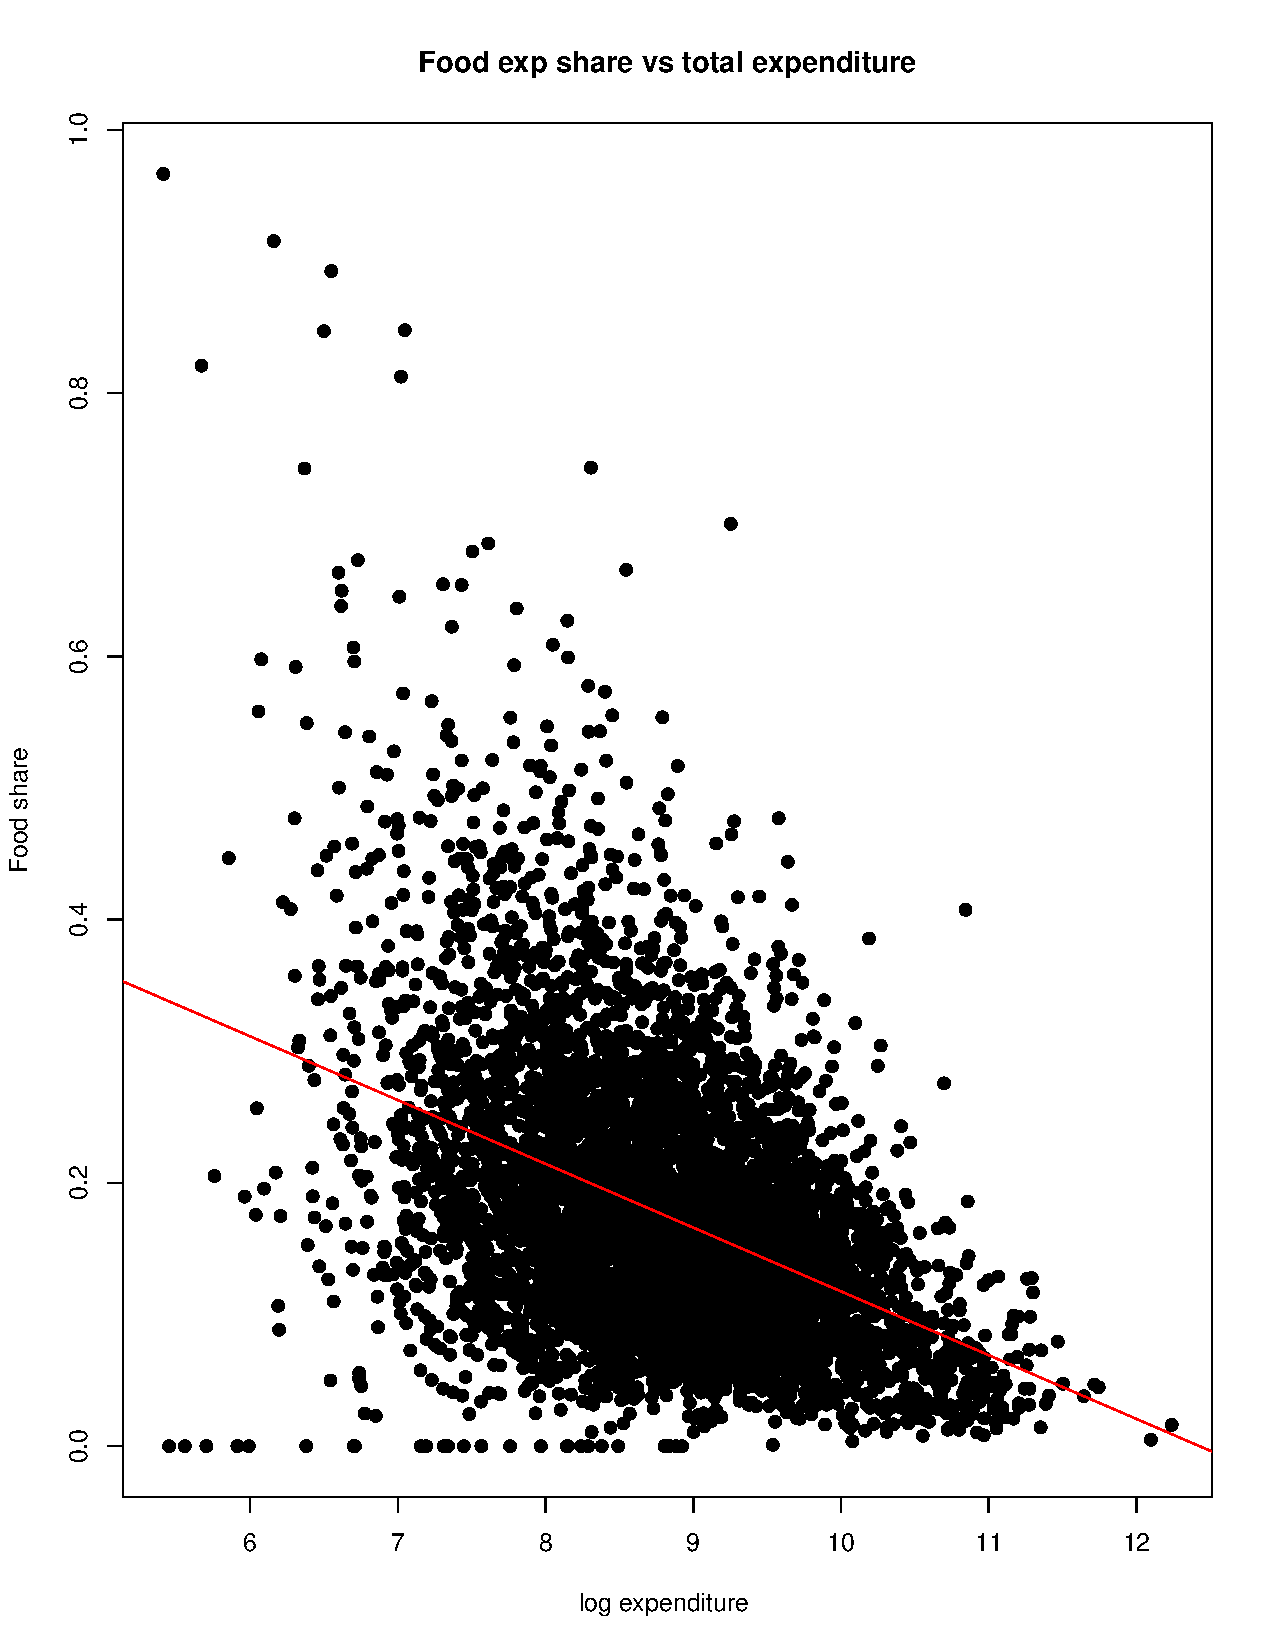
\includegraphics[width=.7\textwidth]{engle1.pdf}	

{\tiny Data source: BLS Consumer Expenditure Survey data}

\end{column}
\begin{column}{0.5\textwidth}
\begin{itemize}
	\item If we plotted total food expenditure (rather than the expenditure share), the heteroscedasticity would go in the other direction.
\end{itemize}
\end{column}
\end{columns}
\end{frame}



\begin{frame}{Heteroscedasticity vs. Correlation}
\begin{itemize}
	\item Recall that we defined the homoscedasticity assumption as:\[
	Var\left(\boldsymbol{\varepsilon} \right) =\sigma^2 {\bf I}
	\]
	this assumption has two aspects:
	\begin{enumerate}
		\item The disturbance for each observation has the same variance
		\item Imposing zero correlation between disturbances for different observations
	\end{enumerate}

	\item The terminology can be misleading here, because what people refer to as ``heteroscedasticity-robust''
	standard errors (the variance estimators on the previous slide) are robust to violations of 1 but not 2. 

	\item We need to do a bit more to estimate standard errors in a way that is robust to correlated data. 

\end{itemize}
\end{frame}


\begin{frame}{Correlation I}
\begin{itemize}
	\item The baseline assumptions of the linear regression framework imply that
	the disturbances are uncorrelated across observations.  There are many ways for this to be violated. 
	\begin{itemize}
		\item Example 1: we might have county-level data for a regression and be concerned
		that different counties within a given state have correlated disturbances because
		all counties are subject to the same (unobserved) state-level policies.
		\item Example 2: time series data (asset prices), and we are worried that some unobserved
		factors within the disturbances are serially correlated
		\item Example 3: county level data again, and we are worried about geographically
		correlated factors such as weather. 
	\end{itemize}
\end{itemize}
\end{frame}


\begin{frame}{Correlation II}
 Different correlation patterns call for different estimators of $\boldsymbol{\Sigma}$, the variance of ${\bf b}_{OLS}$
	Some common alternatives to the no-correlation baseline:
\begin{enumerate}
	\item Clustered standard errors, when there is correlation between observations
	within well-defined groups, but no correlation between observations in different groups. 
	\item Newey-West standard errors (and extensions) to deal with serial correlation
	in time series data.
	\item Conley-Newey-West standard errors that allow for correlation in multiple dimensions
	(especially popular in the context of spatially explicit models).
\end{enumerate}
\end{frame}


\begin{frame}{What is Clustering?}
Suppose we want to relax our i.i.d. assumption:
\begin{itemize}
\item Each observation $i$ is a \alert{villager} and each group $g$ is a \alert{village}
\item Each observation $i$ is a \alert{student} and each group $g$ is a \alert{class}.
\item Each observation $t$ is a \alert{year} and each entity $i$ is a \alert{state}.
\item Each observation $t$ is a \alert{week} and each entity $i$ is a \alert{shopper}.
\end{itemize}
We might expect that $\operatorname { Cov } (u_{g1},u_{g2},\ldots,u_{gN}) \neq 0 \rightarrow$ independence is a bad assumption. 
\end{frame}

\begin{frame}{Clustering: Intuition}
The groups (villages, classrooms, states) are independent of one another, but within each group we can allow for arbitrary correlation.
\begin{itemize}
\item If correlation is within an individual over time we call it \alert{serial correlation} or \alert{autocorrelation}
\item Just like in time-series$\rightarrow$ we have fewer effective independent observations in our sample.
\item Asymptotics now about the number of groups $G \rightarrow \infty$ not observations $N \rightarrow \infty$
\end{itemize}
\end{frame}


\begin{frame}{Clustering I}
\begin{itemize}
	\item Suppose data are organized into distinct groups $g=1,2,\dots,G$. Let $g\left(i\right)$
	be the group identity of observation $i$. 
	\begin{itemize}
		\item e.g., with county-level data, we have $g\left(Manhattan\right)=NY$.
	\end{itemize}


	\medskip
	\item We assume $\E\left[\varepsilon_i \varepsilon_j\right]=0$ as long as $g\left(i\right)\ne g\left(j\right)$,
	and we do not restrict the correlation $\E\left[\varepsilon_i \varepsilon_j\right]$
	for observations within the same group.

	\medskip
	\item Intuition: the linear regression framework with no correlation in observations will overstate
	the precision of our estimates. If we add another observation within a cluster, and that observation
	is highly correlated with the other observations, it's not actually as good as adding another independent observation. 
\end{itemize}
\end{frame}

\begin{frame}{Clustering II}
\begin{itemize}
	\item Recall the sandwich formula for standard errors:\[
		n^{-1} \E\left[{\bf x}_i {\bf x}'_i\right]^{-1} \V\left[{\bf x}_i \varepsilon_i \right] \E\left[{\bf x}_i {\bf x}'_i\right]^{-1}.
	\]

	\item The estimator for the middle part without clustering was\[
	{\bf \V}\left[{\bf x}_i \varepsilon_i \right] = n^{-1} \sum_{i} {\bf x}_i {\bf x}'_i  e_i^2
	\]

	\item With clustering, it will be \[
	{\bf V}_{clu} = n^{-1} \sum_{i=1}^{n}\sum_{j=1}^{n} {\bf x}_i\,  {\bf x}'_j \, e_i\, e_j \cdot {\mathbb{I}}\left[(i,j) \in \text{Group}_g \right]
	\]
	where the ${\bf I}$ function is 1 when $i,j$ come from the same group and zero otherwise.

\end{itemize}
\end{frame}



\begin{frame}{Clustering III}
\begin{itemize}
	\item The cluster-robust estimate of standard errors will be consistent as the number of groups 
	gets large.

	\item Note that this estimator adds extra terms (covariance terms) to the estimate of variance,
	so this is going to make standard errors larger as long as covariances $\E\left[\varepsilon_i \varepsilon_j\right]$ are positive. 

	\item Thus, if standard formulas are used in the presence of cluster-correlated disturbances, 
	standard errors will be too small.

	\item Statistical software packages typically make it easy to compute cluster-robust errors.
	
	\item Clustering often makes a {\bf huge} difference in standard errors.

\end{itemize}
\end{frame}

% \begin{frame}{Correlation III}

%  Consider the cluster-robust estimator of the ``meat'' part of the sandwich estimator: \[
% 	{\bf V}_{clu} = n^{-1} \sum_{i=1}^{n}\sum_{j=1}^{n} {\bf x}_i \, {\bf x}'_j \,  e_i \, e_j\, {\mathbb{I}}\left[g\left(i\right)==g\left(j\right)\right]
% 	\]

% \medskip
%  For Conley-Newey-West standard errors (where there is correlation between ``nearby'' observations),
% 	procedure is similar.

% \medskip
% 	 The difference is that instead of the 1/0 indicator function for ${\bf I}$, we will have a 
% 	weighting (or kernel) function which takes on values $\approx 1$ for ``nearby'' observations and goes to zero for
% 	observations that are far apart.


% \end{frame}


\begin{frame}{Clustering Derviation}
Begin by stacking up observations in each group $\mathbf{y}_{g }  = [y_{g1},\ldots,y_{g n_g}]$, we can write OLS three ways:
\begin{align*}
y_{ig } &= x_{ig}' \beta + \varepsilon_{ig}\\
\mathbf{y}_{g } &= \mathbf{X}_{g} \beta + \boldsymbol{\varepsilon}_{g}\\
\mathbf{Y} &= \mathbf{X} \beta + \boldsymbol{\varepsilon}
\end{align*}
All of these are equivalent:
\begin{align*}
\widehat {  \beta  } &= \left( \sum _ { g = 1 } ^ { G } \sum _ { i = 1 } ^ { n _ { g } } x _ { i g }' { x } _ { i g } \right) ^ { - 1 } \left( \sum _ { g = 1 } ^ { G } \sum _ { i = 1 } ^ { n _ { g } } x _ { i g }' y _ { i g } \right)\\
\widehat {  \beta  }  &=  \left(  \sum _ { g = 1 } ^ { G } \mathbf{X}_g' \mathbf{X}_g \right)^{-1} \left(  \sum _ { g = 1 } ^ { G } \mathbf{X}_g' \mathbf{y}_g \right)\\
\widehat {  \beta  }  &=  \left( \mathbf{X}' \mathbf{X} \right)^{-1} \left(   \mathbf{X}' \mathbf{Y} \right)\\
\end{align*}
\end{frame}

\begin{frame}{Clustering Derivation (Continued)}
The error terms have covariance within each cluster $g$ as:
\begin{align*}
 \boldsymbol{\Sigma}_ { g } = \mathbb { E } \left( \boldsymbol{\varepsilon} _ { g }  \boldsymbol{ \varepsilon } _ { g } ^ { \prime } \mid \boldsymbol { X } _ { g } \right)
\end{align*}

In order to calculate $\widehat{V}_{\widehat{\beta}}$ we replace the covariance matrix $\mathbf{D}$ with $\Omega$ and consider an estimator $\widehat{\Omega}_n$. We exploit \alert{independence across clusters}:
\begin{align*}
\operatorname { var } \left( \left( \sum _ { g = 1 } ^ { G } \boldsymbol { X } _ { g } ^ { \prime } \boldsymbol{\varepsilon}_{ g } \right) \mid \boldsymbol { X } \right) = \sum _ { g = 1 } ^ { G } \operatorname { var } \left( \boldsymbol { X } _ { g } ^ { \prime } \boldsymbol{\varepsilon} _ { g } | \boldsymbol { X } _ { g } \right)
= \sum _ { g = 1 } ^ { G } \boldsymbol { X } _ { g } ^ { \prime } \mathbb { E } \left( \boldsymbol{\varepsilon} _ { g } \boldsymbol{\varepsilon}_ { g } ^ { \prime } | \boldsymbol { X } _ { g } \right) \boldsymbol { X } _ { g }
= \sum _ { g = 1 } ^ { G } \boldsymbol { X } _ { g } ^ { \prime } \boldsymbol { \Sigma } _ { g } \mathbf { X } _ { g } 
 \equiv \Omega_N
\end{align*}
And an estimate of the variance:
\begin{align*}
\boldsymbol { V } _ { \widehat { \boldsymbol { \beta } } } = \operatorname { var } ( \widehat { \boldsymbol { \beta } } \mid  \boldsymbol { X } )
= \left( \mathbf { X } ^ { \prime } \mathbf { X } \right) ^ { - 1 } \boldsymbol { \Omega } _ { n } \left( \mathbf { X } ^ { \prime } \mathbf { X } \right) ^ { - 1 }
\end{align*}
\end{frame}



\begin{frame}{Clustered SE's}
\begin{align*}
\widehat { \boldsymbol { V } } _ { OLS } ^ { \mathrm { CR } 1 } = \left( \boldsymbol { X } ^ { \prime } \boldsymbol { X } \right) ^ { - 1 } \left( \sum _ { g = 1 } ^ { G } \boldsymbol { X } _ { g } ^ { \prime } \boldsymbol { e }_ { g }  \boldsymbol { e }_ { g } ^ { \prime } \boldsymbol { X } _ { g } \right) \left( \boldsymbol { X } ^ { \prime } \boldsymbol { X } \right) ^ { - 1 }\\
\widehat { \boldsymbol { V } } _ { OLS } ^ { \mathrm { CR } 3 } = \left( \boldsymbol { X } ^ { \prime } \boldsymbol { X } \right) ^ { - 1 } \left( \sum _ { g = 1 } ^ { G } \boldsymbol { X } _ { g } ^ { \prime } \widetilde { \boldsymbol { e } } _ { g }  \widetilde { \boldsymbol { e } } _ { g } ^ { \prime } \boldsymbol { X } _ { g } \right) \left( \boldsymbol { X } ^ { \prime } \boldsymbol { X } \right) ^ { - 1 }
\end{align*}
\begin{itemize}
\item Can replace  $\mathbf{e}_g  \rightarrow \tilde { \mathbf{e}}_g $ for leave-one out like $HC3$ (these are called $CR3$).
\end{itemize}
\end{frame}


\begin{frame}[fragile]{Clustering in R}
\begin{lstlisting}
feols(y~ x1 + x2, data=df, vcov=~group_id )
feols(y~ x1 + x2, data=df, vcov=~group_id+time_id)
\end{lstlisting}
\end{frame}



\begin{frame}{Most Asked PhD Student Econometric Question}
 How should I cluster my standard errors?
\begin{itemize}
\item Heck if I know.
\item This is very problem specific
\item It matters a lot $\rightarrow$ standard errors can get orders of magnitude larger.
\item Do you believe across group independence or not? [this is the only thing that matters]
\item If you include \alert{fixed effects} probably you need at least clustering at that level.
\end{itemize}
\end{frame}



\begin{frame}{Bootstrap I}
\begin{itemize}
	\item Another approach to estimating the standard errors of ${\bf b}_{OLS}$
	is the {\bf bootstrap}

	\item The basic idea:
	\begin{enumerate}
		\item Simulate a new data set (same number of observations) by sampling (with replacement) from the original data set

		\item Estimate ${\bf b}_{OLS,s}$ for the new data set.

		\item Repeat lots of times, resulting in a bunch of different estimates of ${\bf b}_{OLS,s}$, say $s=1,\dots,10000$

		\item Look at the variance of the ${\bf b}_{OLS,s}$ estimates 
		across the various simulated data sets. This is your estimate of $\boldsymbol{\Sigma}$, or $Var\left({\bf b}_{OLS}\right)$
	\end{enumerate}

\end{itemize}
\end{frame}


\begin{frame}{Bootstrap II}
\begin{itemize}
	\item The bootstrap's main appeal is that it can provide a better finite-sample
	approximation of the distribution of the parameter estimates.
	\begin{itemize}
		\item Note that the Eicker-Huber-White standard errors estimates are \emph{consistent}, but
		not generally \emph{unbiased} in finite samples
		\item The bootstrap is probably worth trying if you're ever working with
		 non-linear estimators (which can be consistent but are typically not unbiased in finite samples). 
	\end{itemize}

	\medskip
	\item Also, it can potentially deliver good estimates of standard errors even with 
	correlated errors, but this depends on the version of the bootstrap (see {\bf block bootstrap}).
	 Exploring formally the  conditions under which the bootstrap works well is beyond our scope. 
\end{itemize}
\end{frame}


\end{document}